
\documentclass[aps,pra,reprint,showpacs,nofootinbib,superscriptaddress]{revtex4-1}
%%%%%%%%%%%%%%%%%%%%%%%%%%%%%%%%%%%%%%%%%%%%%%%%%%%%%%%%%%%%%%%%%%%%%%%%%%%%%%%%%%%%%%%%%%%%%%%%%%%%%%%%%%%%%%%%%%%%%%%%%%%%%%%%%%%%%%%%%%%%%%%%%%%%%%%%%%%%%%%%%%%%%%%%%%%%%%%%%%%%%%%%%%%%%%%%%%%%%%%%%%%%%%%%%%%%%%%%%%%%%%%%%%%%%%%%%%%%%%%%%%%%%%%%%%%%
%    Q-circuit version 2
%    Copyright (C) 2004  Steve Flammia & Bryan Eastin
%    Last modified on: 9/16/2011
%
%    This program is free software; you can redistribute it and/or modify
%    it under the terms of the GNU General Public License as published by
%    the Free Software Foundation; either version 2 of the License, or
%    (at your option) any later version.
%
%    This program is distributed in the hope that it will be useful,
%    but WITHOUT ANY WARRANTY; without even the implied warranty of
%    MERCHANTABILITY or FITNESS FOR A PARTICULAR PURPOSE.  See the
%    GNU General Public License for more details.
%
%    You should have received a copy of the GNU General Public License
%    along with this program; if not, write to the Free Software
%    Foundation, Inc., 59 Temple Place, Suite 330, Boston, MA  02111-1307  USA

% Thanks to the Xy-pic guys, Kristoffer H Rose, Ross Moore, and Daniel Müllner,
% for their help in making Qcircuit work with Xy-pic version 3.8.  
% Thanks also to Dave Clader, Andrew Childs, Rafael Possignolo, Tyson Williams,
% Sergio Boixo, Cris Moore, Jonas Anderson, and Stephan Mertens for helping us test 
% and/or develop the new version.

\usepackage{xy}
\xyoption{matrix}
\xyoption{frame}
\xyoption{arrow}
\xyoption{arc}

\usepackage{ifpdf}
\ifpdf
\else
\PackageWarningNoLine{Qcircuit}{Qcircuit is loading in Postscript mode.  The Xy-pic options ps and dvips will be loaded.  If you wish to use other Postscript drivers for Xy-pic, you must modify the code in Qcircuit.tex}
%    The following options load the drivers most commonly required to
%    get proper Postscript output from Xy-pic.  Should these fail to work,
%    try replacing the following two lines with some of the other options
%    given in the Xy-pic reference manual.
\xyoption{ps}
\xyoption{dvips}
\fi

% The following resets Xy-pic matrix alignment to the pre-3.8 default, as
% required by Qcircuit.
\entrymodifiers={!C\entrybox}

\newcommand{\bra}[1]{{\left\langle{#1}\right\vert}}
\newcommand{\ket}[1]{{\left\vert{#1}\right\rangle}}
    % Defines Dirac notation. %7/5/07 added extra braces so that the commands will work in subscripts.
\newcommand{\qw}[1][-1]{\ar @{-} [0,#1]}
    % Defines a wire that connects horizontally.  By default it connects to the object on the left of the current object.
    % WARNING: Wire commands must appear after the gate in any given entry.
\newcommand{\qwx}[1][-1]{\ar @{-} [#1,0]}
    % Defines a wire that connects vertically.  By default it connects to the object above the current object.
    % WARNING: Wire commands must appear after the gate in any given entry.
\newcommand{\cw}[1][-1]{\ar @{=} [0,#1]}
    % Defines a classical wire that connects horizontally.  By default it connects to the object on the left of the current object.
    % WARNING: Wire commands must appear after the gate in any given entry.
\newcommand{\cwx}[1][-1]{\ar @{=} [#1,0]}
    % Defines a classical wire that connects vertically.  By default it connects to the object above the current object.
    % WARNING: Wire commands must appear after the gate in any given entry.
\newcommand{\gate}[1]{*+<.6em>{#1} \POS ="i","i"+UR;"i"+UL **\dir{-};"i"+DL **\dir{-};"i"+DR **\dir{-};"i"+UR **\dir{-},"i" \qw}
    % Boxes the argument, making a gate.
\newcommand{\meter}{*=<1.8em,1.4em>{\xy ="j","j"-<.778em,.322em>;{"j"+<.778em,-.322em> \ellipse ur,_{}},"j"-<0em,.4em>;p+<.5em,.9em> **\dir{-},"j"+<2.2em,2.2em>*{},"j"-<2.2em,2.2em>*{} \endxy} \POS ="i","i"+UR;"i"+UL **\dir{-};"i"+DL **\dir{-};"i"+DR **\dir{-};"i"+UR **\dir{-},"i" \qw}
    % Inserts a measurement meter.
    % In case you're wondering, the constants .778em and .322em specify
    % one quarter of a circle with radius 1.1em.
    % The points added at + and - <2.2em,2.2em> are there to strech the
    % canvas, ensuring that the size is unaffected by erratic spacing issues
    % with the arc.
\newcommand{\measure}[1]{*+[F-:<.9em>]{#1} \qw}
    % Inserts a measurement bubble with user defined text.
\newcommand{\measuretab}[1]{*{\xy*+<.6em>{#1}="e";"e"+UL;"e"+UR **\dir{-};"e"+DR **\dir{-};"e"+DL **\dir{-};"e"+LC-<.5em,0em> **\dir{-};"e"+UL **\dir{-} \endxy} \qw}
    % Inserts a measurement tab with user defined text.
\newcommand{\measureD}[1]{*{\xy*+=<0em,.1em>{#1}="e";"e"+UR+<0em,.25em>;"e"+UL+<-.5em,.25em> **\dir{-};"e"+DL+<-.5em,-.25em> **\dir{-};"e"+DR+<0em,-.25em> **\dir{-};{"e"+UR+<0em,.25em>\ellipse^{}};"e"+C:,+(0,1)*{} \endxy} \qw}
    % Inserts a D-shaped measurement gate with user defined text.
\newcommand{\multimeasure}[2]{*+<1em,.9em>{\hphantom{#2}} \qw \POS[0,0].[#1,0];p !C *{#2},p \drop\frm<.9em>{-}}
    % Draws a multiple qubit measurement bubble starting at the current position and spanning #1 additional gates below.
    % #2 gives the label for the gate.
    % You must use an argument of the same width as #2 in \ghost for the wires to connect properly on the lower lines.
\newcommand{\multimeasureD}[2]{*+<1em,.9em>{\hphantom{#2}} \POS [0,0]="i",[0,0].[#1,0]="e",!C *{#2},"e"+UR-<.8em,0em>;"e"+UL **\dir{-};"e"+DL **\dir{-};"e"+DR+<-.8em,0em> **\dir{-};{"e"+DR+<0em,.8em>\ellipse^{}};"e"+UR+<0em,-.8em> **\dir{-};{"e"+UR-<.8em,0em>\ellipse^{}},"i" \qw}
    % Draws a multiple qubit D-shaped measurement gate starting at the current position and spanning #1 additional gates below.
    % #2 gives the label for the gate.
    % You must use an argument of the same width as #2 in \ghost for the wires to connect properly on the lower lines.
\newcommand{\control}{*!<0em,.025em>-=-<.2em>{\bullet}}
    % Inserts an unconnected control.
\newcommand{\controlo}{*+<.01em>{\xy -<.095em>*\xycircle<.19em>{} \endxy}}
    % Inserts a unconnected control-on-0.
\newcommand{\ctrl}[1]{\control \qwx[#1] \qw}
    % Inserts a control and connects it to the object #1 wires below.
\newcommand{\ctrlo}[1]{\controlo \qwx[#1] \qw}
    % Inserts a control-on-0 and connects it to the object #1 wires below.
\newcommand{\targ}{*+<.02em,.02em>{\xy ="i","i"-<.39em,0em>;"i"+<.39em,0em> **\dir{-}, "i"-<0em,.39em>;"i"+<0em,.39em> **\dir{-},"i"*\xycircle<.4em>{} \endxy} \qw}
    % Inserts a CNOT target.
\newcommand{\qswap}{*=<0em>{\times} \qw}
    % Inserts half a swap gate.
    % Must be connected to the other swap with \qwx.
\newcommand{\multigate}[2]{*+<1em,.9em>{\hphantom{#2}} \POS [0,0]="i",[0,0].[#1,0]="e",!C *{#2},"e"+UR;"e"+UL **\dir{-};"e"+DL **\dir{-};"e"+DR **\dir{-};"e"+UR **\dir{-},"i" \qw}
    % Draws a multiple qubit gate starting at the current position and spanning #1 additional gates below.
    % #2 gives the label for the gate.
    % You must use an argument of the same width as #2 in \ghost for the wires to connect properly on the lower lines.
\newcommand{\ghost}[1]{*+<1em,.9em>{\hphantom{#1}} \qw}
    % Leaves space for \multigate on wires other than the one on which \multigate appears.  Without this command wires will cross your gate.
    % #1 should match the second argument in the corresponding \multigate.
\newcommand{\push}[1]{*{#1}}
    % Inserts #1, overriding the default that causes entries to have zero size.  This command takes the place of a gate.
    % Like a gate, it must precede any wire commands.
    % \push is useful for forcing columns apart.
    % NOTE: It might be useful to know that a gate is about 1.3 times the height of its contents.  I.e. \gate{M} is 1.3em tall.
    % WARNING: \push must appear before any wire commands and may not appear in an entry with a gate or label.
\newcommand{\gategroup}[6]{\POS"#1,#2"."#3,#2"."#1,#4"."#3,#4"!C*+<#5>\frm{#6}}
    % Constructs a box or bracket enclosing the square block spanning rows #1-#3 and columns=#2-#4.
    % The block is given a margin #5/2, so #5 should be a valid length.
    % #6 can take the following arguments -- or . or _\} or ^\} or \{ or \} or _) or ^) or ( or ) where the first two options yield dashed and
    % dotted boxes respectively, and the last eight options yield bottom, top, left, and right braces of the curly or normal variety.  See the Xy-pic reference manual for more options.
    % \gategroup can appear at the end of any gate entry, but it's good form to pick either the last entry or one of the corner gates.
    % BUG: \gategroup uses the four corner gates to determine the size of the bounding box.  Other gates may stick out of that box.  See \prop.

\newcommand{\rstick}[1]{*!L!<-.5em,0em>=<0em>{#1}}
    % Centers the left side of #1 in the cell.  Intended for lining up wire labels.  Note that non-gates have default size zero.
\newcommand{\lstick}[1]{*!R!<.5em,0em>=<0em>{#1}}
    % Centers the right side of #1 in the cell.  Intended for lining up wire labels.  Note that non-gates have default size zero.
\newcommand{\ustick}[1]{*!D!<0em,-.5em>=<0em>{#1}}
    % Centers the bottom of #1 in the cell.  Intended for lining up wire labels.  Note that non-gates have default size zero.
\newcommand{\dstick}[1]{*!U!<0em,.5em>=<0em>{#1}}
    % Centers the top of #1 in the cell.  Intended for lining up wire labels.  Note that non-gates have default size zero.
\newcommand{\Qcircuit}{\xymatrix @*=<0em>}
    % Defines \Qcircuit as an \xymatrix with entries of default size 0em.
\newcommand{\link}[2]{\ar @{-} [#1,#2]}
    % Draws a wire or connecting line to the element #1 rows down and #2 columns forward.
\newcommand{\pureghost}[1]{*+<1em,.9em>{\hphantom{#1}}}
    % Same as \ghost except it omits the wire leading to the left. 

% \usepackage{tikz}
% \usetikzlibrary{quantikz}
\usepackage{graphicx,comment}
\usepackage{amsfonts}
\usepackage{amsmath,amssymb}
%\usepackage[varg]{txfonts}
\usepackage{bm}
\usepackage{color}
% \usepackage{epstopdf}
% \epstopdfsetup{outdir=./Figures/}
% \usepackage{epsfig}
% \usepackage[font=small,
%   justification=justified,
%   format=plain]{caption} % 'format=plain' avoids hanging indentation
% \usepackage{subfig}
%\usepackage{float}
%\usepackage[compat=1.1.0]{tikz-feynman}
%\usepackage{a4wide,amssymb,float}
\usepackage{verbatim}
\usepackage{hyperref}
\usepackage{multirow}
\usepackage[table,xcdraw]{xcolor}
\usepackage{tabularx}
\usepackage{wrapfig}
% \usepackage{ragged2e}
% \usepackage{subcaption}
% \usepackage[skip=2pt]{caption}
\hypersetup{
     colorlinks   = true,
     citecolor    = blue
}
\usepackage{lineno}
% \usepackage[thicklines]{cancel}
\usepackage{color, colortbl}
% \definecolor{LightCyan}{rgb}{0.88,1,1}
% \usepackage{url}
% \usepackage{dcolumn}
%
%  package for subfiles
%
\usepackage{subfiles}
% %
% \usepackage{lineno}
\newcommand{\todo}[1]{\textcolor{red}{#1}}    
% \usepackage{graphicx}
\def\ho{\tilde{\omega}}
\def\tio{\hat{\omega}}
\def\tp{\tilde{p}}
%%%%%%%%%%%%%%%%%%%%%%%%%%%%%%%%%%%%%%%%%%%%%%%%
\def\de{\partial}
\def\a{\alpha}
\def\b{\beta}
\def\g{\gamma}
\def\G{\Gamma}
\def\d{\delta}
\def\D{\Delta}
\def\e{\eta}
\def\f{\phi}{\rm }
\def\la{\lambda}
\def\La{\Lambda}
\def\k{\kappa}
\def\m{\mu}
\def\n{\nu}
\def\r{\rho}
%\def\o{\omega}
\def\p{\pi}
\def\s{\sigma}
\def\S{\Sigma}
\def\t{\tau}
\def\ep{\epsilon}
\def\th{\theta}
\def\z{\zeta}
\def\x{\chi}
%%%%%%%%%%%%%%%%%%%%%%%%%%%%%%%%%%%%%%%%%%%%%%%%%
\def\be{\begin{equation}}
 \def\ee{\end{equation}}
 \def\bea{\begin{eqnarray}}
 \def\eea{\end{eqnarray}}
 % ------- Define Greek Lowercase --------
 \def\a{\alpha}
 \def\b{\beta}
 \def\g{\gamma}
 \def\d{\delta}
 %\def\o{\omega}
 \def\s{\sigma}
 % ------- Define Greek Uppercase --------
\def\G{\Gamma}
\def\L{\Lambda}

\def\ho{\tilde{\omega}}
\def\tio{\hat{\omega}}
\def\tp{\tilde{p}}
\newcommand{\fr}{\frac}
\newcommand{\pr}{\prime}
\newcommand{\pp}{{\prime \prime}}
%\renewcommand{\CancelColor}{\color{red}}
%\newcommand{\stkout}[1]{\ifmmode\text{\sout{\ensuremath{#1}}}\else\sout{#1}\fi}
\def\pa{\partial}
\def\A{\mathcal{A}}
\def\B{\mathcal{B}}
\def\F{\mathcal{F}}
\def\H{\mathcal{H}}
\def\K{\mathcal{K}}
\def\N{\mathcal{N}}
\def\O{\mathcal{O}}
\def\R{\mathcal{R}}
\def\W{\mathcal{W}}
\def\2{\frac{1}{2}}
\def\4{\frac{1}{4}}

\def\ap{a_+}
\def\am{a_-}
%\newcommand{\bra}[1]{\left\langle #1 \right|}
%\newcommand{\ket}[1]{\left| #1 \right\rangle}
\newcommand{\expect}[1]{\langle {#1} \rangle}
\newcommand{\braket}[2]{\left\langle #1 \vert #2 \right\rangle}

\def\nn{\nonumber}


% \def\np#1{{Nucl.\ Phys.\ B \bf #1}}
% \def\pl#1{{Phys.\ Lett.\ B \bf #1}}
% \def\PLA#1{{Phys.\ Lett.\ A \bf #1}}
% \def\PR#1{{Phys.\ Rev.\ D \bf #1}}
% \def\PRL#1{{Phys.\ Rev.\ Lett.\ \bf #1}}
% \def\cm#1{{Commun.\ Math.\ Phys.\ \bf #1}}
% \def\mpl#1{{Mod.\ Phys.\ Lett.\ A \bf #1}}
% \def\cpc#1{{Comp.\ Phys.\ Comm.\ \bf #1}}
% \def\anp#1{{Annals Phys.\ \bf #1}}
% \def\rmp#1{{Rev.\ Mod.\ Phys.\ \bf #1}}
% \def\cqg#1{{Class.\ Quant.\ Grav.\ \bf #1}}
% \def\gen{\mathrm{g}}

% \catcode`\@=11

% %       This causes equations to be numbered by section

% %\@addtoreset{equation}{section}
% %\def\theequation{\arabic{equation}}
% %\def\theequation{\thesection.\arabic{equation}}

% \def\@normalsize{\@setsize\normalsize{15pt}\xiipt\@xiipt
% \abovedisplayskip 14pt plus3pt minus3pt%
% \belowdisplayskip \abovedisplayskip
% \abovedisplayshortskip  \z@ plus3pt%
% \belowdisplayshortskip  7pt plus3.5pt minus0pt}
% \def\small{\@setsize\small{13.6pt}\xipt\@xipt
% \abovedisplayskip 13pt plus3pt minus3pt%
% \belowdisplayskip \abovedisplayskip
% \abovedisplayshortskip  \z@ plus3pt%
% \belowdisplayshortskip  7pt plus3.5pt minus0pt
% \def\@listi{\parsep 4.5pt plus 2pt minus 1pt
%             \itemsep \parsep
%             \topsep 9pt plus 3pt minus 3pt}}

% \def\underline#1{\relax\ifmmode\@@underline#1\else
%         $\@@underline{\hbox{#1}}$\relax\fi}
% \@twosidetrue \relax


% \catcode`@=12

% %       set page size
% %\evensidemargin 0.0in \oddsidemargin 0.0in \topmargin -0.2in
% %\textwidth 6.4in \textheight 8.9in \headsep .50in

% %       reset section commands

% %       reset section commands

% \catcode`\@=11
% \def\lover#1{
%       \raisebox{1.3ex}{\rlap{$\leftarrow$}} \raisebox{ 0ex}{$#1$}}
% \def\section{\@startsection{section}{1}{\z@}{3.5ex plus 1ex minus
%   .2ex}{2.3ex plus .2ex}{\large\bf}}
% %\def\thesection{\arabic{section}.}
% %\def\thesubsection{\arabic{section}-\arabic{subsection}.}
% %       reset the page style
% \def\FERMIPUB{}
% \def\FERMILABPub#1{\def\FERMIPUB{#1}}
% \def\ps@headings{\def\@oddfoot{}\def\@evenfoot{}
% \def\@oddhead{\hbox{}\hfill
%         \makebox[.5\textwidth]{\raggedright\ignorespaces --\thepage{}--
%         \hfill }}
% \def\@evenhead{\@oddhead}
% \def\subsectionmark##1{\markboth{##1}{}}
% }

% \ps@headings

% \catcode`\@=12

%%%%%%%%%%%%%%%%%%%%%%%%%%%%%%%%%%%%%%%%%%%%%%%%%%%%%%%%%%%%%%%%%%%%%%%%
\linenumbers
\begin{document}
\title{Profiling Field Theory Application Performance on Quantum Computers Using Cycle Benchmarking and Randomized Compiling}
%\title{Studying the Ising Model Trotterization with Cycle Benchmarking and Randomized Compiling}
%
{\footnote{ \textbf{SHOULD THIS GO IN THE ACKNOWLEDGMENTS? DOES IT BELONG HERE ON PAGE 1} This manuscript has been authored by UT-Battelle, LLC, under Contract No. DE-AC0500OR22725 with the U.S. Department of Energy. The United States Government retains and the publisher, by accepting the article for publication, acknowledges that the United States Government retains a non-exclusive, paid-up, irrevocable, world-wide license to publish or reproduce the published form of this manuscript, or allow others to do so, for the United States Government purposes. The Department of Energy will provide public access to these results of federally sponsored research in accordance with the DOE Public Access Plan.}}

\author{project team}
%\author{K\"ubra Yeter-Aydeniz }
%\email{yeteraydenik@ornl.gov}
%\affiliation{Physics Division, Oak Ridge National Laboratory,
%  Oak Ridge, TN 37831, USA}
%\affiliation{Computational Sciences and Engineering Division, Oak Ridge National %Laboratory,
%  Oak Ridge, TN 37831, USA}




%\author{Alexander F. Kemper}
%\affiliation{Department of Physics, North Carolina State University, Raleigh, North %Carolina 27695, USA}
%\email{akemper@ncsu.edu}

%\author{Raphael C.\ Pooser}
%\email{pooserrc@ornl.gov}
%\affiliation{Computational Sciences and Engineering Division, Oak Ridge National %Laboratory,
%  Oak Ridge, TN 37831, USA}

%\author{Patrick Dreher}
%\affiliation{North Carolina State University, Raleigh, North Carolina 27695, USA}


\date{\today}

\begin{abstract}
 The current generation of noisy intermediate scale quantum computing systems now offer a sufficient number of qubits to begin modelling the performance of simple field theory algorithms on these hardware platforms.  To address the problems of errors arising from these noisy qubits there has been a concerted effort to study how the qubit placement of these qubits on the chip impacts 
\end{abstract}

\maketitle

\subfile{sections/Introduction}


\section{Physics Model}
\label{sec:model}
We study the transverse Ising model (TIM) with open boundary conditions (OBC) with system Hamiltonian 
\be
H_{\text{OBC}}=-J\sum_{i=1}^{N_s-1} X_i X_{i+1} - h_T \sum_{i=1}^{N_s} Z_i \label{eq:H_OBC}
\ee
where $\sigma_i$ for $\sigma \in \{X,Z\}$ are the Pauli matrices calculated for the specific site, $N_s$ is the number of sites, $J$ is the nearest neighbor coupling (hopping) and $h_T$ is the on-site energy. In this work, we will study the case with $N_s=4$, $J=0.02$ and $h_T=1$.

\section{Cycle Benchmarking and Randomized Compiling}
\label{sec:cb}
We used the cycle benchmarking protocol studied in \cite{Erhard2019} and TrueQ software developed by Quantum Benchmark.

The system can be evolved in time using the complex exponential of the Hamiltonian:
\begin{equation}
\label{eqtimeevolveexact}
\hat{U}(t) = e^{- i t \hat{H}}.
\end{equation}
Following Refs. \cite{Lloyd1073,GustafsonIsing},
the Trotter approximation %must be used because the %nearest-neighbor coupling terms do not %commute with the onsite field strength %terms the operator in Eq. %\ref{eqtimeevolveexact}. This %approximation leads to the following %expression for the time evolution %operation 
is applied to the evolution operator 
with the explicit form:
\begin{equation}
\label{eqsuzuki}
\hat{U}(t;N) = \Big(\hat{U}_1(t / N; h_t) \hat{U}_2(t / N; J)\Big)^N + \mathcal{O}(t^2 / N)
\end{equation}
where $N$ is the number of Trotter steps to be implemented, $(\delta t)$ is the Trotter step size
\begin{equation}
\label{eqtfieldevo}
\hat{U}_1(\delta t; h_t) = e^{-i h_T \delta t \sum_{i = 1}^{4} \hat{\sigma}^z_i },
\end{equation}
and
\begin{equation}
\label{eqhoppingevo}
\hat{U}_2(\delta t; J) = e^{-i J \delta t \sum_{i = 1}^{3} \hat{\sigma}^x_i \hat{\sigma}^x_{i+1}}.
\end{equation}
The operators defined in Eqs. \ref{eqtfieldevo}  and \ref{eqhoppingevo} can be expressed as a combination of the following two quantum circuits:
\begin{equation}
\label{eqtfieldevocirc}
\hat{U}_{1}(\delta t; h_t) = 
\begin{aligned}
\Qcircuit @C=-1.3em @R=-0.5cm @! {
& \gate{R_z^{h_t}(\delta t)} & \qw\\
& \gate{R_z^{h_t}(\delta t)} & \qw\\
& \gate{R_z^{h_t}(\delta t)} & \qw\\
& \gate{R_z^{h_t}(\delta t)} & \qw\\
}
\end{aligned}
\end{equation}
and
\begin{equation}
\label{eqhoppingevocirc}
\hat{U}_2(\delta t; J) =  \begin{gathered}\Qcircuit @C=-1.3em @R=-0.5cm @! {
& \ctrl{1} & \gate{R_x^J(\delta t)} & \ctrl{1} & \qw & \qw & \qw & \qw \\
& \targ & \qw                    & \targ & \ctrl{1} & \gate{R_x^J(\delta t)} & \ctrl{1} & \qw \\
& \ctrl{1} & \gate{R_x^J(\delta t)} & \ctrl{1} & \targ & \qw & \targ & \qw \\ 
& \targ & \qw                    & \targ & \qw & \qw & \qw & \qw \\
}
\end{gathered},
\end{equation}
where $R_x^J(\delta t) = e^{i J \delta t \hat{\sigma}^x}$ and $R_z^{h_t}(\delta t) = e^{i \delta t h_t \hat{\sigma}^z}$. We selected the qubits 0, 1, 2, 3 on Boeblingen so that we could observe the occupation index output over time using a consistent set of qubits for all measurements.




\begin{equation}
    \begin{gathered}
    \Qcircuit @R=1em @C=1em {
    & \ctrl{1} & \gate{e^{-i \delta t J \sigma^x}} & \ctrl{1} &  \qw & \qw & \qw  & \qw & \qw & \qw &\qw \\
    & \targ & \qw & \targ & \ctrl{1} & \gate{e^{-i \delta t J \sigma^x}} & \ctrl{1}  & \qw & \qw & \qw&\qw\\
    & \qw & \qw & \qw & \targ & \qw & \targ & \ctrl{1} & \gate{e^{-i \delta t J \sigma^x}} & \ctrl{1}&\qw\\
    & \qw & \qw & \qw  & \qw & \qw & \qw & \targ & \qw & \targ &\qw\\
    }
    \end{gathered}
\end{equation}



\section{Methodology} 

The experiments were run on IBM Q Boeblingen hardware on days 01/23-31/2021 for three times a day such that 
\begin{itemize}
    \item Run 1 of the day was run around 6:30 am after the first calibration of the device, 
    \item Run 2 of the day was run around 3:00 pm which is about 12 hours after the first calibration of the device,  
    \item Run 3 of the day started around 8:30 pm after second calibration of the device.
\end{itemize} 
We chose 3 qubit layouts to run the cycle benchmarking protocol to decide about which qubit layout provides the best performance for the open boundary conditions (OBC) Ising model Hamiltonian time evolution using Trotterization. These qubit layouts are
\begin{itemize}
    \item $[q_0,q_1,q_2,q_3]=[0,1,2,3]$ which is a layout in the upper left corner of the device,
    \item $[q_0,q_1,q_2,q_3]=[6,7,11,12]$ which is a layout in the middle of the device,
    \item $[q_0,q_1,q_2,q_3]=[16,17,18,19]$ which is a layout in the lower right corner of the device.
\end{itemize}



The experiments were run IBM Q Boeblingen device which has the qubit layout as seen in Fig.~\ref{fig:BoeblingenLayout}. 
\begin{figure}[ht!]
    % \centering
    % \includegraphics[width=2.2\columnwidth]{final_plot.pdf}
    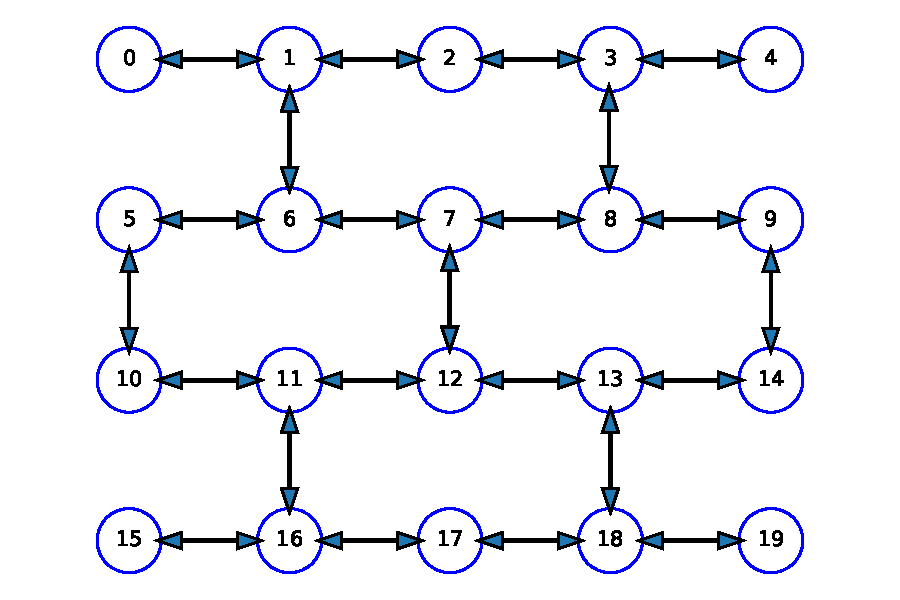
\includegraphics[scale=0.45]{QubitLayoutBoeblingen.pdf}
    \caption{IBM Q Boeblingen device qubit layout.}
    \label{fig:BoeblingenLayout}
\end{figure}








\section{Benchmarking Measurements}

\subsection{Transverse Ising Model}

\subsection{Cycle Benchmarking}
The measured process infidelities ($e_F$) obtained using CB protocol are presented in Fig.~\ref{fig:CB} for qubit layouts $[0,1,2,3],[6,7,12,11],[16,17,18,19]$, runs 1, 2, and 3 between days 01/23-31/2021 for cycles demonstrated in Fig.~\ref{fig:BoeblingenCycles}.
\begin{figure*}[ht!]
    % \centering
    % \includegraphics[width=2.2\columnwidth]{final_plot.pdf}
    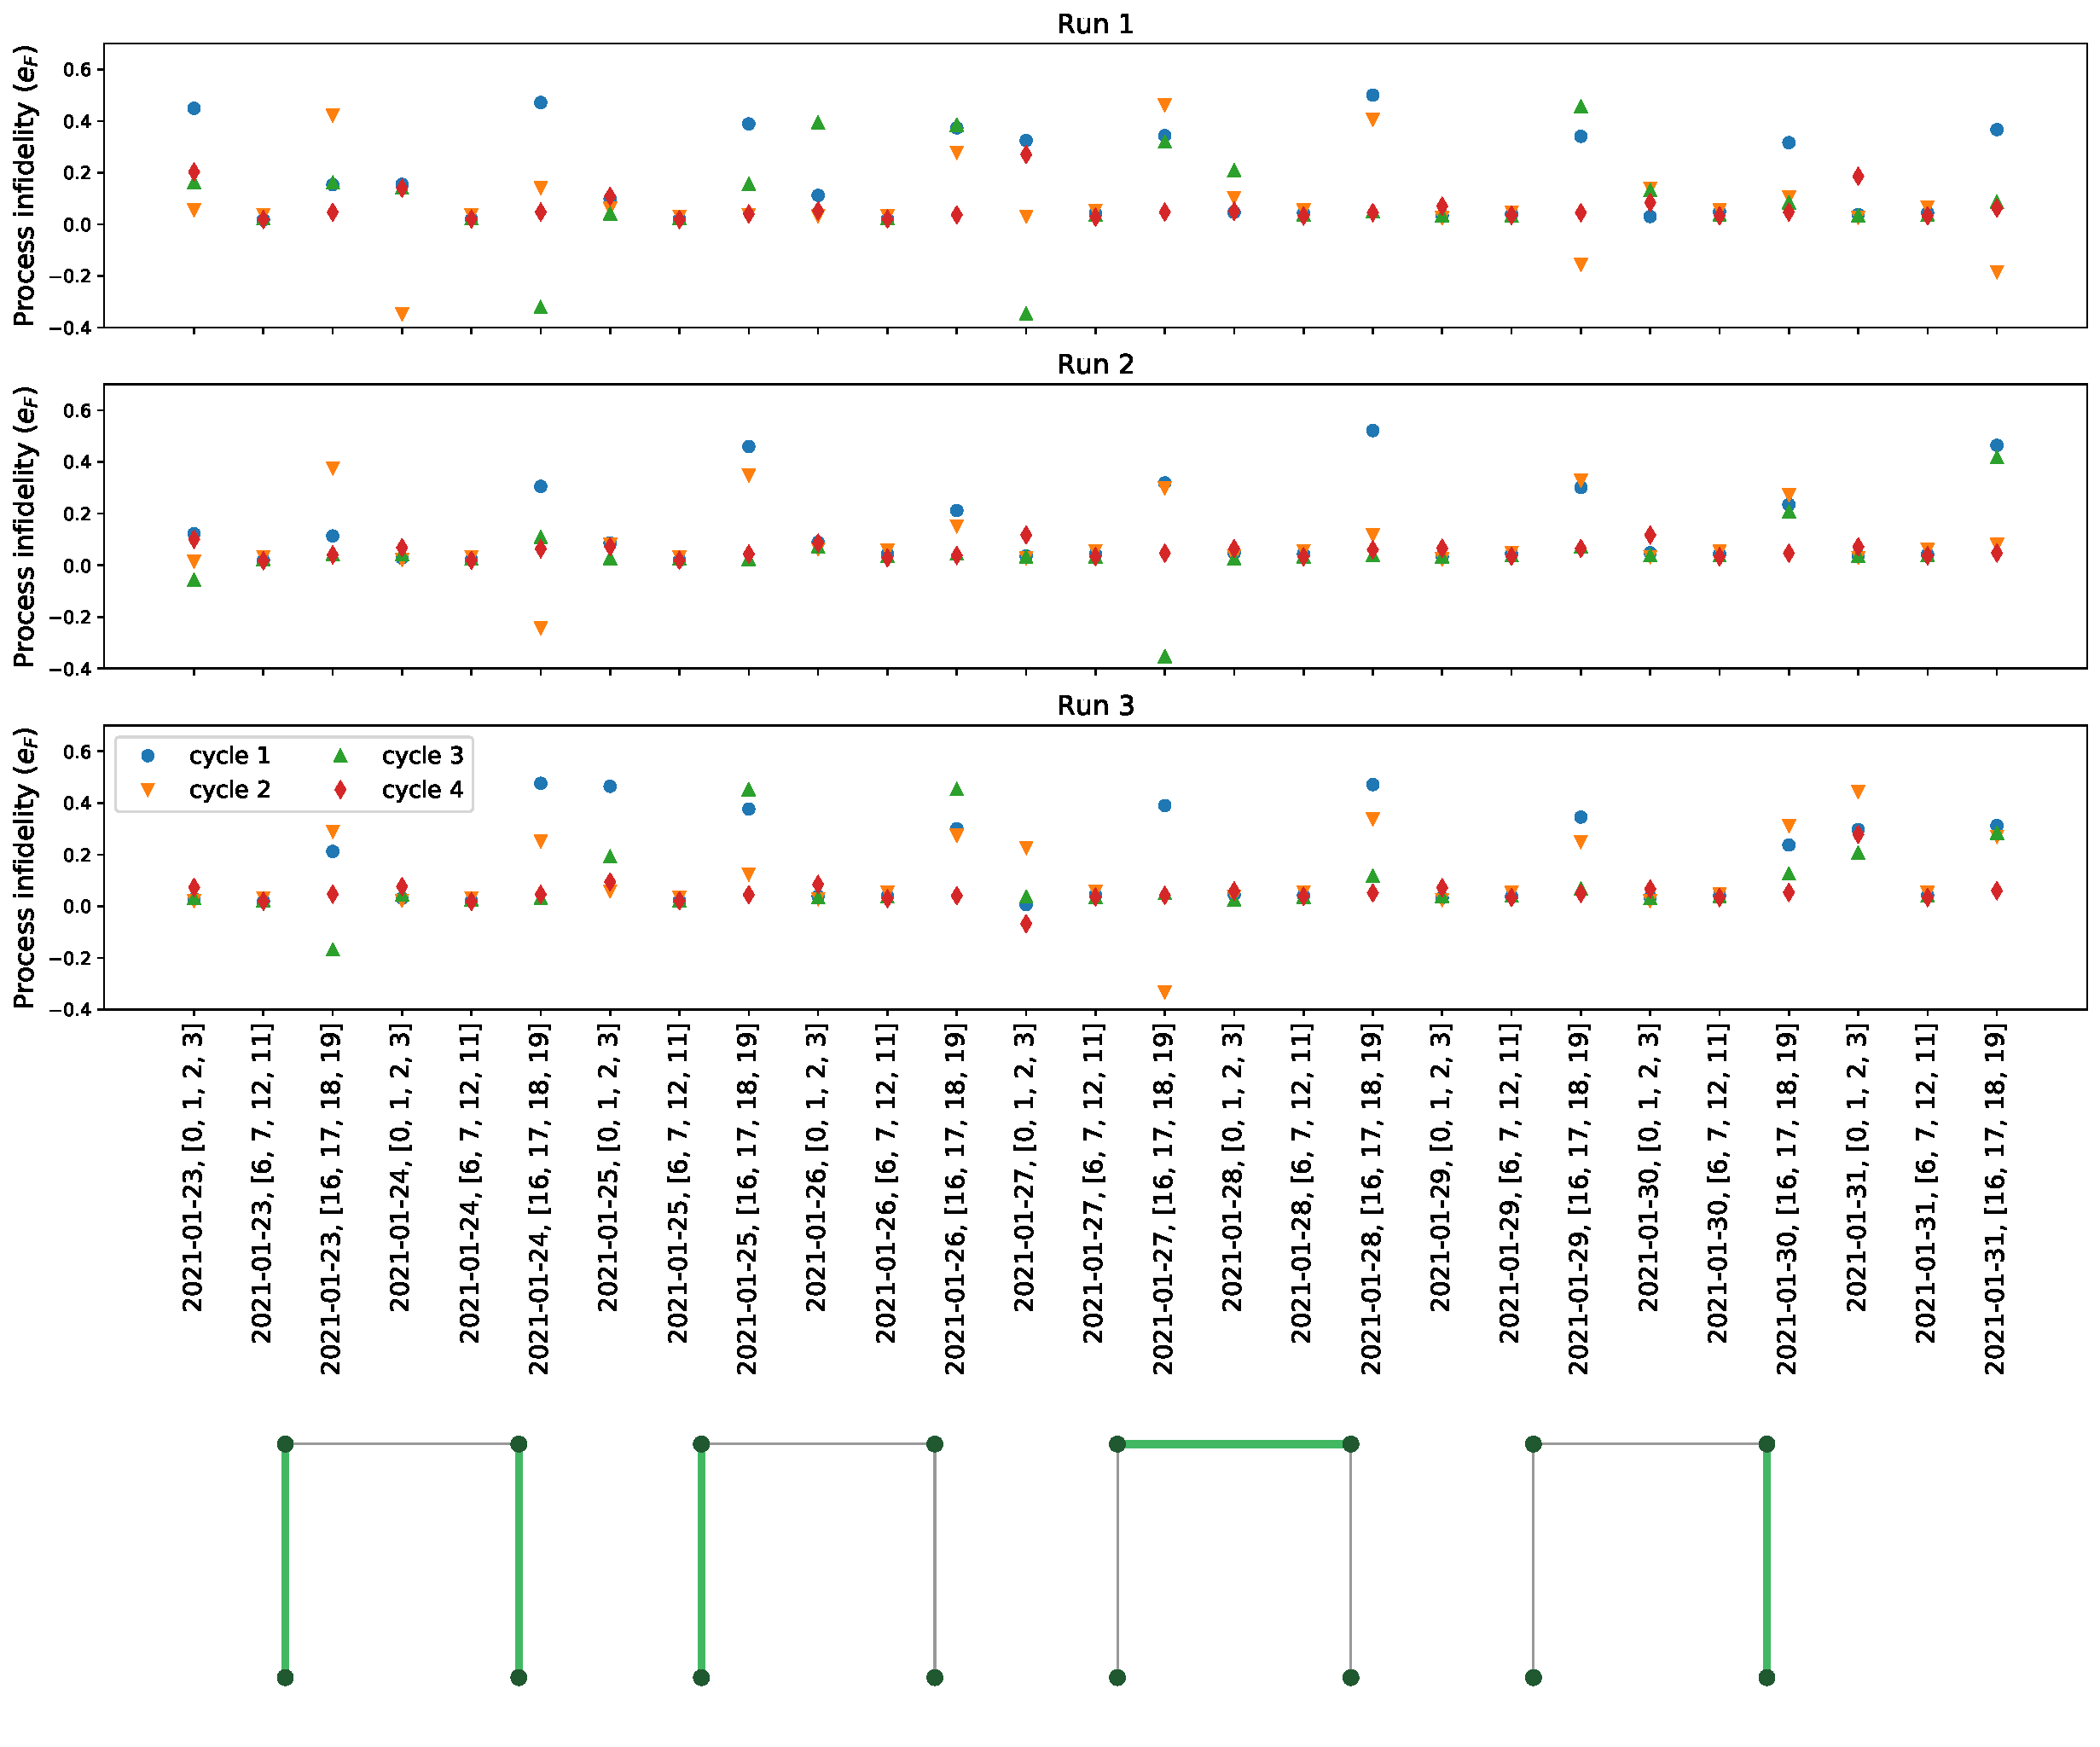
\includegraphics[scale=0.42]{CBForEachDayEachRunEachLayout.pdf}
    \caption{Process infidelity ($e_F$) calculated using cycle benchmarking the circuits ran on IBM Q Boeblingen hardware for layouts $[0,1,2,3],[6,7,12,11],[16,17,18,19]$, runs 1, 2, and 3 between days 01/23-31/2021 are presented.}
    \label{fig:CB}
\end{figure*}

The cycle benchmarking data was obtained using the following variables. For each cycle of interest we used sequence lengths of 2, 10, and 22, respectively. The sequence length refers to the number of times the cycle of interest appears apart from state inversion. The number of random circuits used in each sequence length is 48. Each of these circuits at each sequence length were run $N_\text{shots}=128$ times. 

The process infidelity is estimated from the average value of the individual Pauli infidelities.


\subsubsection{Process Infidelity Measurements}
The process infidelity ($e_{F}$) was calculated using cycle benchmarking method for CNOT cycles seen in Fig.~\ref{fig:BoeblingenCycles}. Each row in Fig.~\ref{fig:BoeblingenCycles} corresponds to the CNOT cycles  studied for each qubit layout. There are four cycles studied for each qubit layout and we label each of these unique cycle as cycle 1, cycle 2, cycle 3 and cycle 4, respectively from left to right.
\begin{figure}[ht!]
    % \centering
    % \includegraphics[width=2.2\columnwidth]{final_plot.pdf}
    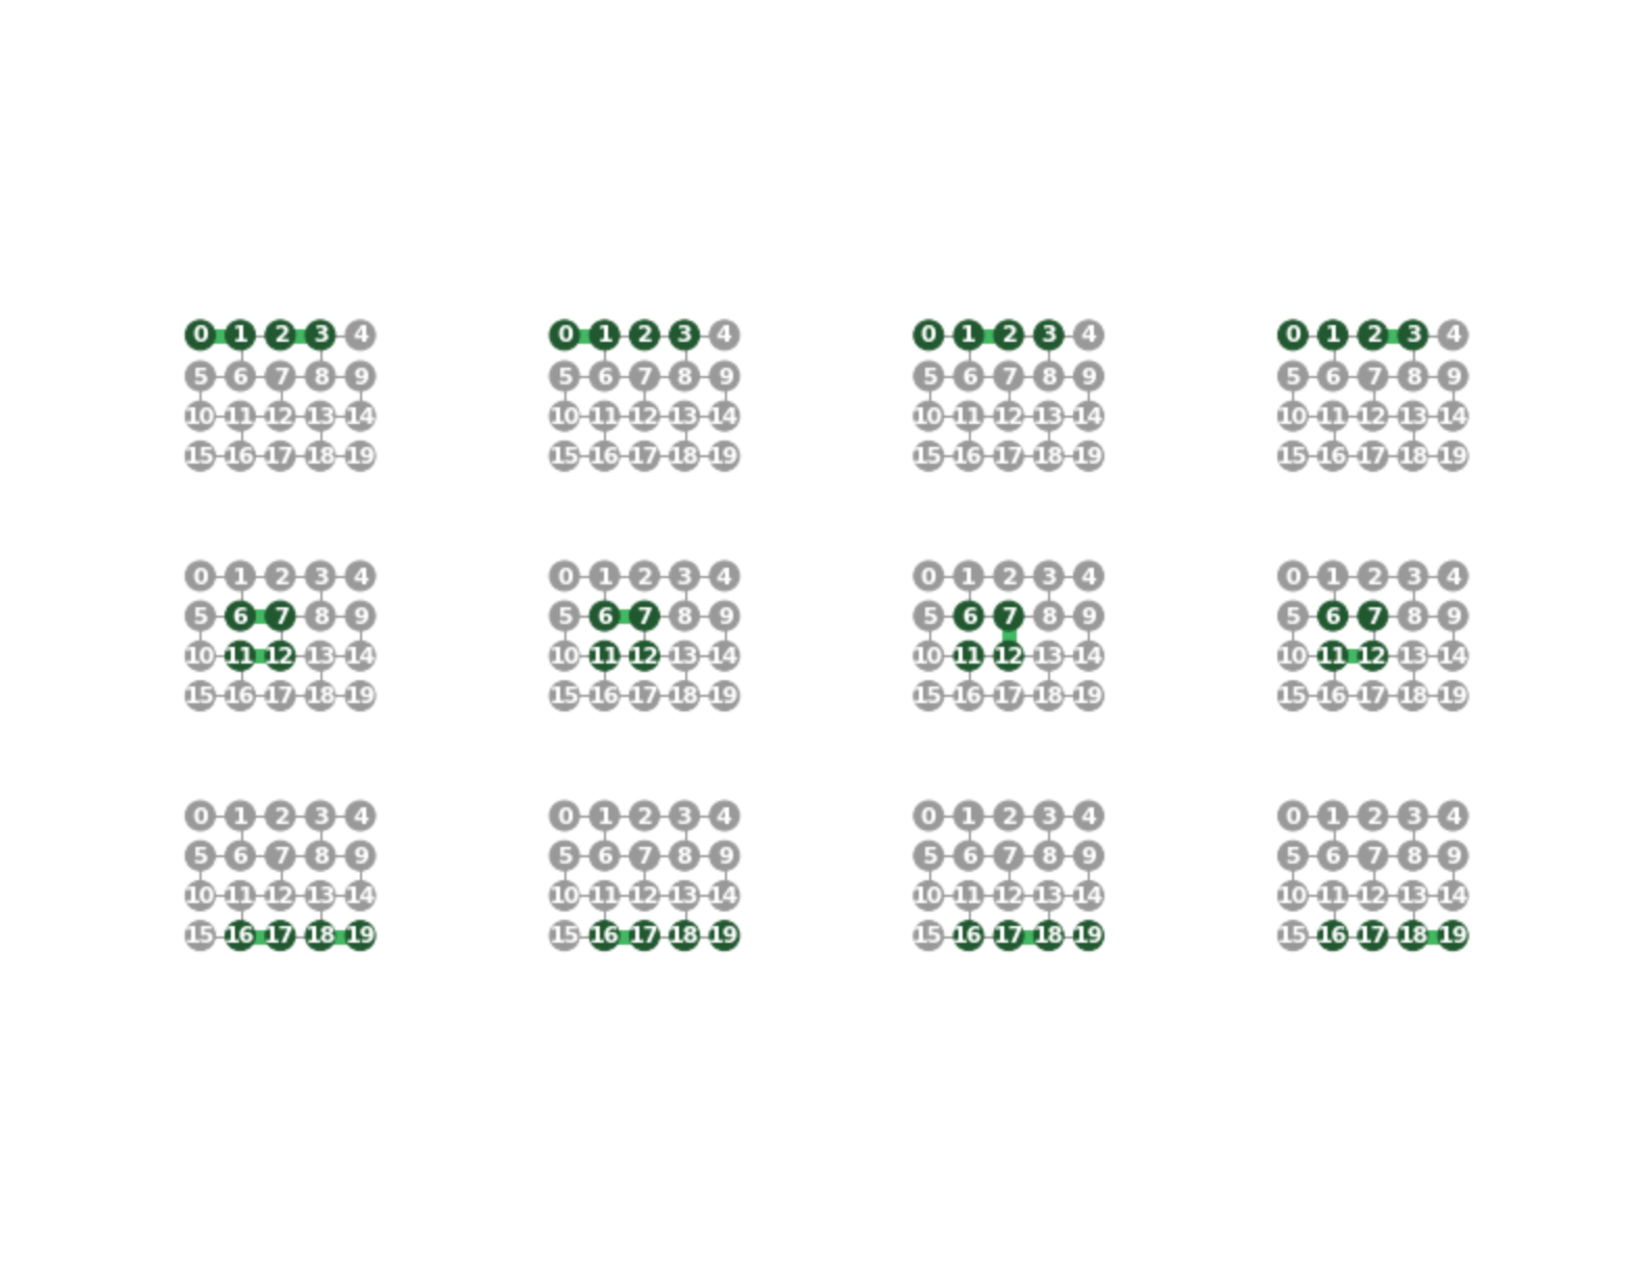
\includegraphics[scale=0.4]{BoeblingenCycles.pdf}
    \caption{The CNOT cycles used to calculate the process infidelities on IBM Q Boeblingen device.}
    \label{fig:BoeblingenCycles}
\end{figure}






\subsubsection{Quantum Capacity (QCap) Bound}
In Fig.s~\ref{fig:QCapCirc1}, \ref{fig:QCapCirc2}, \ref{fig:QCapCirc1and2} we present the QCap bound ($e_{IU}$) values calculated as a function of number of Trotter steps for circuits 1, circuit 2 and circuits 1 and 2 together. The data in Fig.~\ref{fig:QCapCirc1} demonstrates that qubit layout [6, 7, 12, 11] on Boeblingen quantum hardware performs the best for almost all runs and in each day of the experiment for Circuit 1. 

We also studied quantum capacity (QCap) as a function of the number of Trotter steps. QCap is able to estimate an upper bound on the total variational distance (TVD) without a full quantum simulation by characterizing the error rate of each cycle in the circuit and combining the results. This upper bound assumes the circuit is being run under randomized compiling (RC). Under RC, each dressed cycle of a circuit will have a stochastic error model whose process fidelity is estimated directly by CB. In this setting, errors accumulate in a circuit in a predictable way: the process fidelity of the circuit is the product of the process fidelity of each cycle. This parameter is estimated as this product, with error bars derived from standard propagation of uncertainty techniques. {\color{red}{KYA: Cite QB website.}}

We conducted QCap measurements for two quantum circuits as seen in Fig.~\ref{fig:IsingTrotterCircs}. Both of these quantum circuits result in time evolution of a state with $\mathcal{U}=e^{-iH_{\text{OBC}}\tau}$ using Trotterization where $\tau$ is the time interval for one Trotter step.  
\begin{figure*}[!tb]
\[ {\Qcircuit @C=0.5em @R=0.5em {
     \lstick{} & \gate{R_Z(h \tau)} & \multigate{1}{R_{XX}(2 J \tau)} &\qw&\qw  & & & &\\ 
     \lstick{} & \gate{R_Z(h \tau)}  & \ghost{R_{XX}(2 J \tau)} & \multigate{1}{R_{XX}(2 J \tau)}&\qw & & & &\\
     \lstick{} &  \gate{R_Z(h \tau)} & \multigate{1}{R_{XX}(2 J \tau)}&\ghost{R_{XX}(2 J \tau)}&\qw & & & & \\
     \lstick{} &  \gate{R_Z(h \tau)} & \ghost{R_{XX}(2 J \tau)} &\qw&\qw& & & &}}
    { \Qcircuit @C=0.5em @R=0.5em {
     \lstick{} & \gate{R_Z(h \tau)} & \multigate{1}{R_{XX}(2 J \tau)} &\qw&\qw &\qw & \qw\\ 
     \lstick{} & \gate{R_Z(h \tau)}  & \ghost{R_{XX}(2 J \tau)} & \multigate{1}{R_{XX}(2 J \tau)}&\qw&\qw&\qw \\
     \lstick{} &  \gate{R_Z(h \tau)} & \qw&\ghost{R_{XX}(2 J \tau)}&\qw & \multigate{1}{R_{XX}(2 J \tau)}\\
     \lstick{} &  \gate{R_Z(h \tau)} & \qw &\qw&\qw&\ghost{R_{XX}(2 J \tau)}}
}\]
\caption{The quantum circuit for one Trotter step of the time evolution with the open boundary condition Ising model Hamiltonian. We define the quantum circuit in left (right) panel as Circuit 1 (Circuit 2).}
\label{fig:IsingTrotterCircs}
\end{figure*}



\begin{figure*}[ht!]
    % \centering
    % \includegraphics[width=2.2\columnwidth]{final_plot.pdf}
    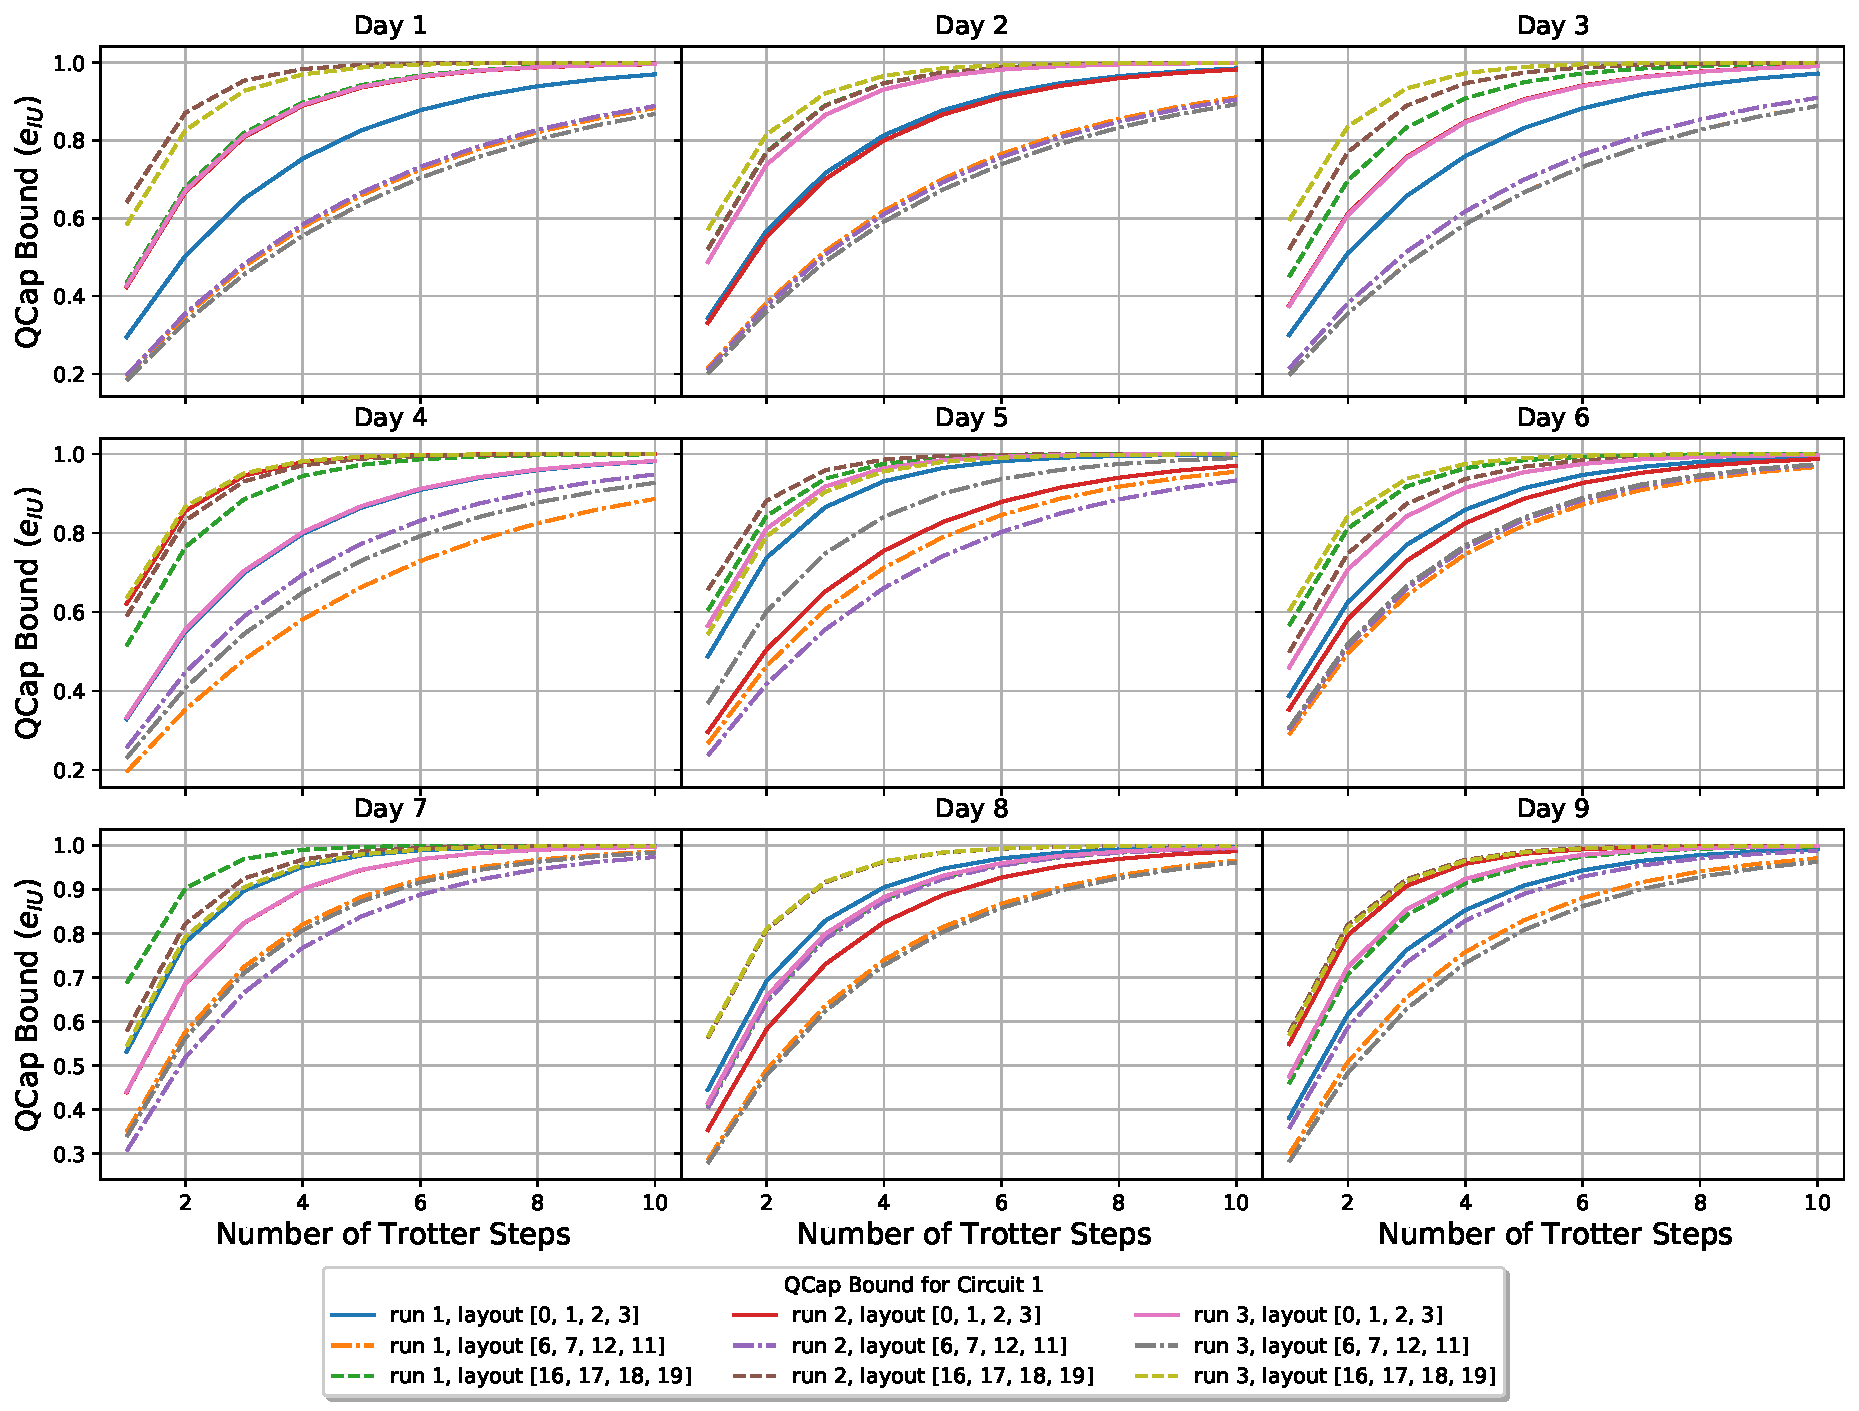
\includegraphics[scale=0.5]{QCapBoundForEachDay_Circ1.pdf}
    \caption{QCap bounds calculated using IBM Q Boeblingen hardware as a function of number of Trotter steps for circuit 1, layouts $[0,1,2,3],[6,7,12,11],[16,17,18,19]$, runs 1, 2, and 3 between days 01/23-31/2021 are presented.}
    \label{fig:QCapCirc1}
\end{figure*}
\begin{figure*}[ht!]
    % \centering
    % \includegraphics[width=2.2\columnwidth]{final_plot.pdf}
    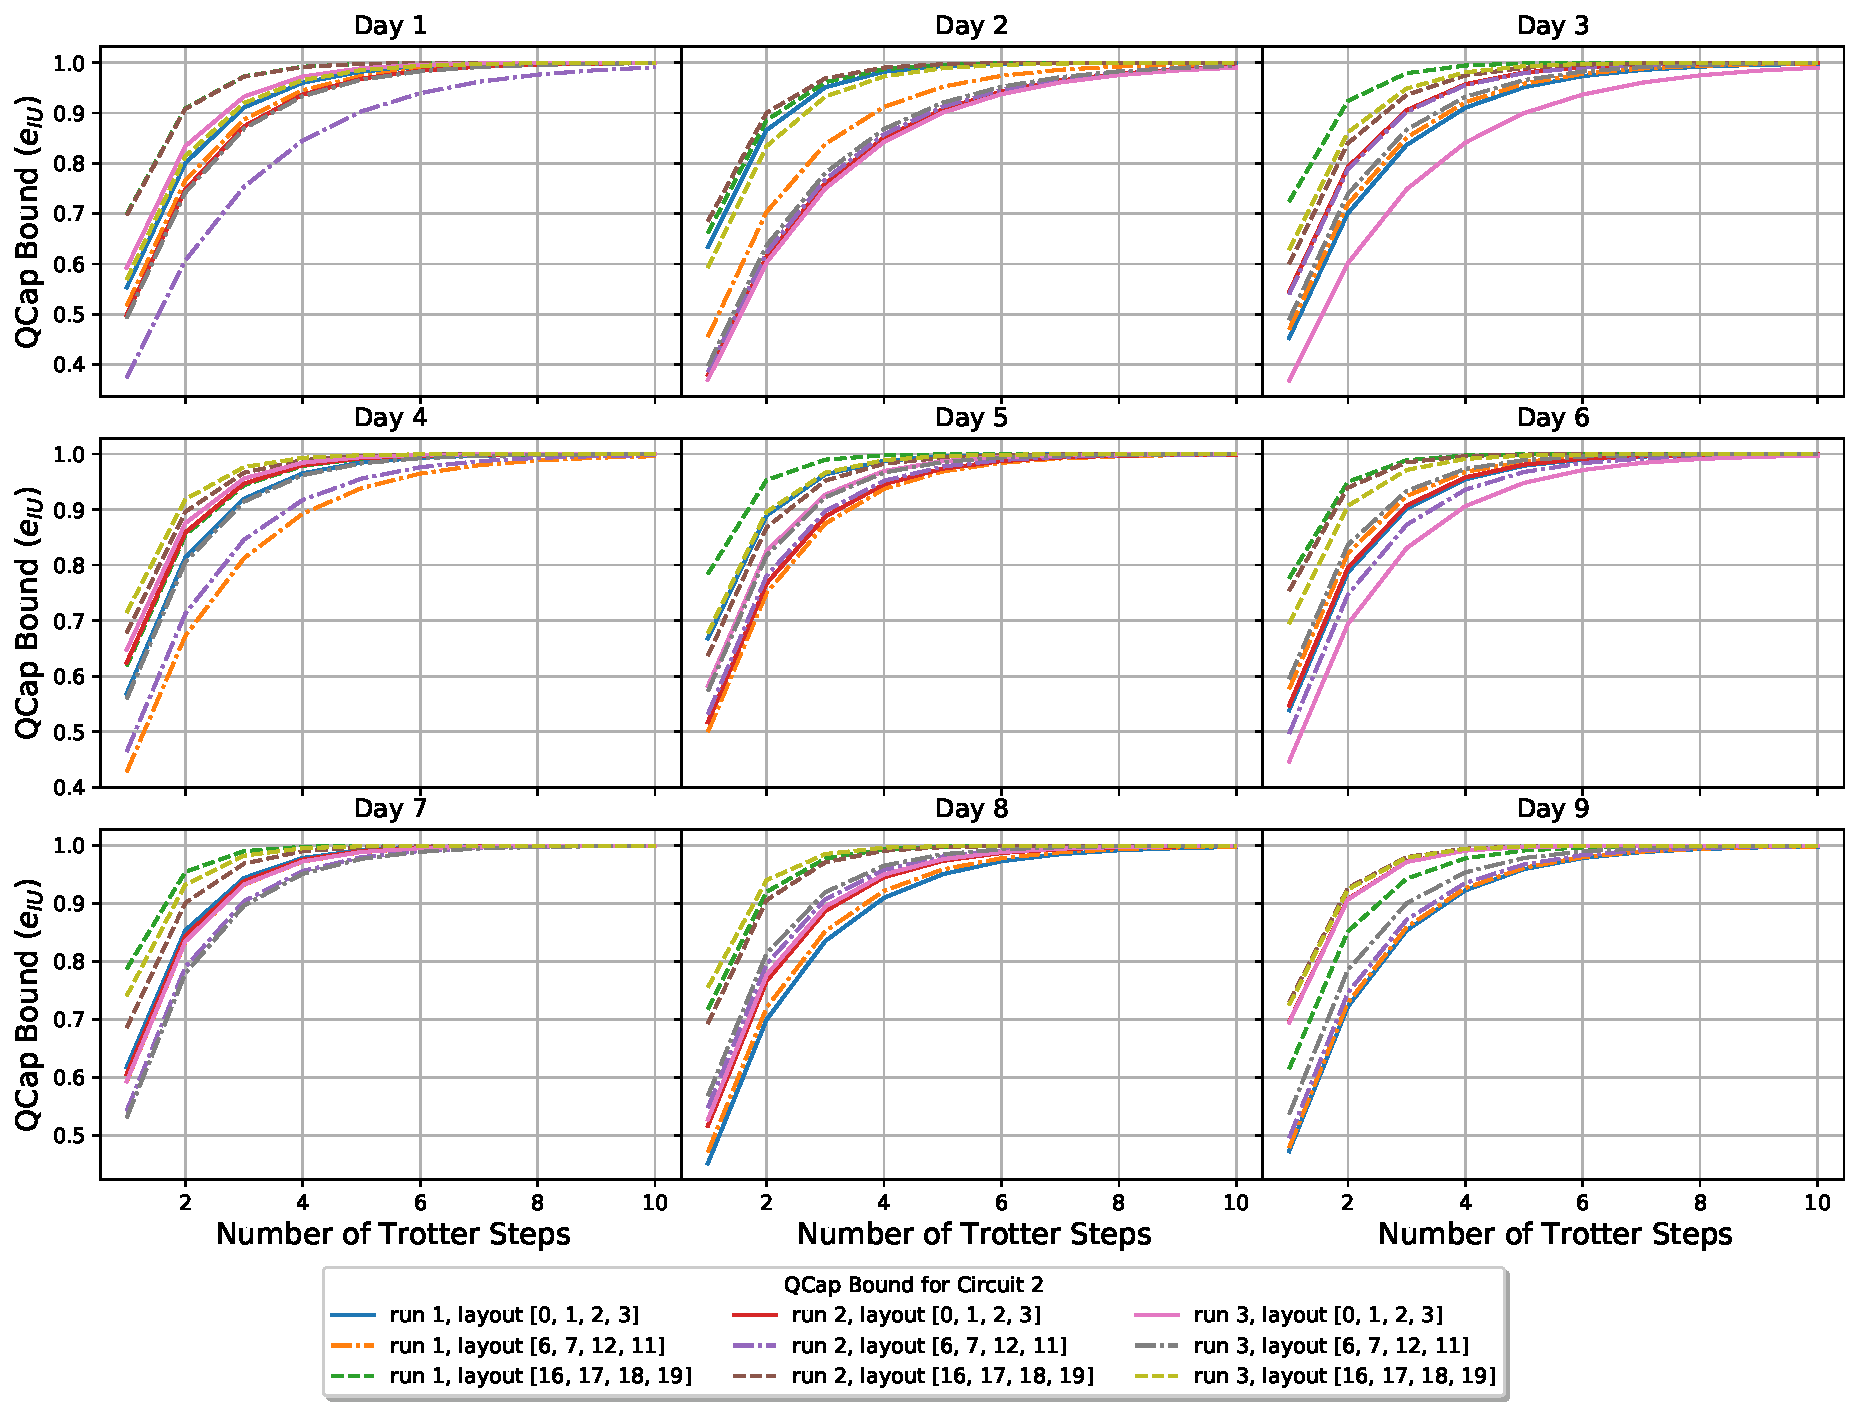
\includegraphics[scale=0.5]{QCapBoundForEachDay_Circ2.pdf}
    \caption{QCap bounds calculated using IBM Q Boeblingen hardware as a function of Trotter steps for circuit 2, layouts $[0,1,2,3],[6,7,12,11],[16,17,18,19]$, runs 1, 2, and 3 between days 01/23-31/2021 are presented.}
    \label{fig:QCapCirc2}
\end{figure*}

\begin{figure*}[ht!]
    % \centering
    % \includegraphics[width=2.2\columnwidth]{final_plot.pdf}
    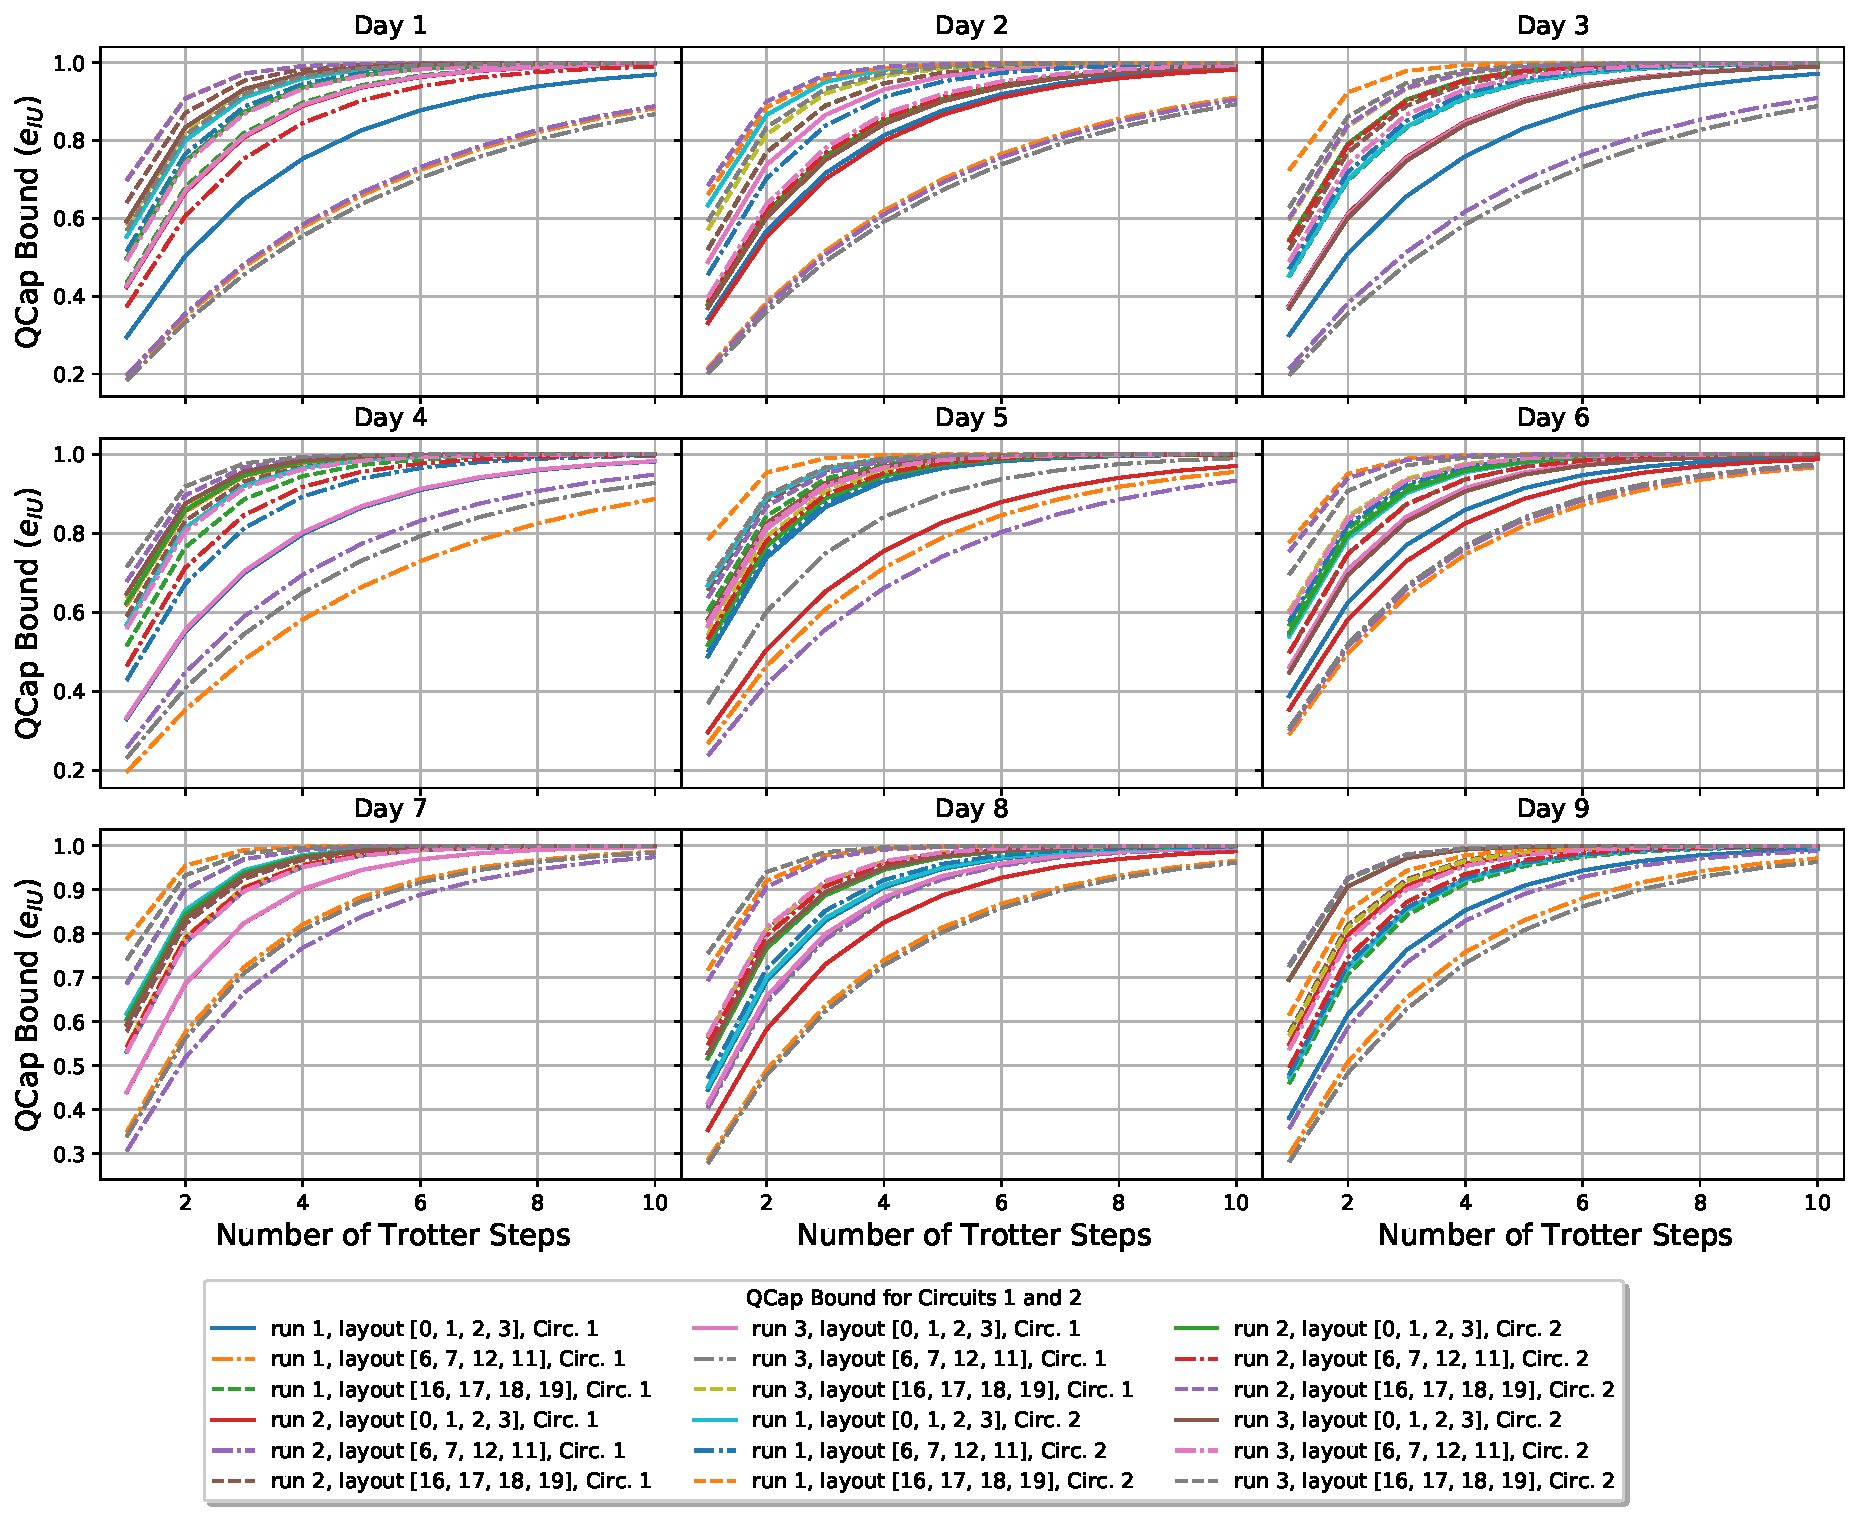
\includegraphics[scale=0.5]{QCapBoundForEachDay_Circ1andCirc2.pdf}
    \caption{QCap bounds calculated using IBM Q Boeblingen hardware as a function of number of Trotter steps for circuit 1 and 2 are compared for layouts $[0,1,2,3],[6,7,12,11],[16,17,18,19]$, runs 1, 2, and 3 between days 01/23-31/2021 are presented.}
    \label{fig:QCapCirc1and2}
\end{figure*}

The parameters used for QCap measurements is as follows. Due to limited access to the dedicated mode on Boeblingen device we use sequence lengths of 4 and 16. The number of random circuits in this case is 30 and each of these circuits were run $N_{\text{shots}}=128$. 
\section{Data Analysis and Discussion}
This is the data analysis section

\begin{table}
  \begin{tabular}{|c|c|c|c|c|c|c|c|c|}
    \hline
    \multirow{2}{*}{CNOT error} &
      \multicolumn{2}{|c}{Q6} &
      \multicolumn{2}{|c}{Q7} &
      \multicolumn{2}{|c}{Q11} &
      \multicolumn{2}{|c|}{Q12} \\
    & IBM & CB & IBM & CB & IBM & CB & IBM & CB \\
    \hline
    Jan 24th  & 1.0 \% & 2.0\% & 3.0\% & 4.0\% & 5.0\% & 6.0\% & 7.0\% & 8.0\%    \\
    \hline
    Jan 25th  & 1.0 \% & 2.0\% & 3.0\% & 4.0\% & 5.0\% & 6.0\% & 7.0\% & 8.0\%    \\
    \hline
    Jan 26th  & 1.0 \% & 2.0\% & 3.0\% & 4.0\% & 5.0\% & 6.0\% & 7.0\% & 8.0\%    \\
    \hline
    Jan 27th  & 1.0 \% & 2.0\% & 3.0\% & 4.0\% & 5.0\% & 6.0\% & 7.0\% & 8.0\%    \\
    \hline
    Jan 28th  & 1.0 \% & 2.0\% & 3.0\% & 4.0\% & 5.0\% & 6.0\% & 7.0\% & 8.0\%    \\
    \hline
    Jan 29th  & 1.0 \% & 2.0\% & 3.0\% & 4.0\% & 5.0\% & 6.0\% & 7.0\% & 8.0\%    \\
    \hline
     Jan 30th  & 1.0 \% & 2.0\% & 3.0\% & 4.0\% & 5.0\% & 6.0\% & 7.0\% & 8.0\%    \\
    \hline
    Jan 31st  & 1.0 \% & 2.0\% & 3.0\% & 4.0\% & 5.0\% & 6.0\% & 7.0\% & 8.0\%    \\
    \hline
  \end{tabular}
\end{table}

\section{Summary}
\section{Acknowledgments}


We acknowledge useful discussions with Ian Hincks and Dar Dahlen. The quantum circuits were drawn using Q-circuit package \cite{QCircuit}.
KYA and RCP were supported by the Quantum Information Science Enabled Discovery (QuantISED) for High Energy Physics program at ORNL under FWP number ERKAP61 and used resources of Oak Ridge Leadership Computing Facility located at ORNL, which is supported by the Office of Science of the Department of Energy under contract No. DE-AC05-00OR22725.
 The authors acknowledge use of the IBM Q for this work. The views expressed are those of the authors and do not reflect the official policy or position of IBM or the IBM Q team. The authors also acknowledge the use of TrueQ software by Quantum Benchmark.


\twocolumngrid
% \Floatbarrier

\begin{thebibliography}{23}%
\makeatletter
\providecommand \@ifxundefined [1]{%
 \@ifx{#1\undefined}
}%
\providecommand \@ifnum [1]{%
 \ifnum #1\expandafter \@firstoftwo
 \else \expandafter \@secondoftwo
 \fi
}%
\providecommand \@ifx [1]{%
 \ifx #1\expandafter \@firstoftwo
 \else \expandafter \@secondoftwo
 \fi
}%
\providecommand \natexlab [1]{#1}%
\providecommand \enquote  [1]{``#1''}%
\providecommand \bibnamefont  [1]{#1}%
\providecommand \bibfnamefont [1]{#1}%
\providecommand \citenamefont [1]{#1}%
\providecommand \href@noop [0]{\@secondoftwo}%
\providecommand \href [0]{\begingroup \@sanitize@url \@href}%
\providecommand \@href[1]{\@@startlink{#1}\@@href}%
\providecommand \@@href[1]{\endgroup#1\@@endlink}%
\providecommand \@sanitize@url [0]{\catcode `\\12\catcode `\$12\catcode
  `\&12\catcode `\#12\catcode `\^12\catcode `\_12\catcode `\%12\relax}%
\providecommand \@@startlink[1]{}%
\providecommand \@@endlink[0]{}%
\providecommand \url  [0]{\begingroup\@sanitize@url \@url }%
\providecommand \@url [1]{\endgroup\@href {#1}{\urlprefix }}%
\providecommand \urlprefix  [0]{URL }%
\providecommand \Eprint [0]{\href }%
\providecommand \doibase [0]{http://dx.doi.org/}%
\providecommand \selectlanguage [0]{\@gobble}%
\providecommand \bibinfo  [0]{\@secondoftwo}%
\providecommand \bibfield  [0]{\@secondoftwo}%
\providecommand \translation [1]{[#1]}%
\providecommand \BibitemOpen [0]{}%
\providecommand \bibitemStop [0]{}%
\providecommand \bibitemNoStop [0]{.\EOS\space}%
\providecommand \EOS [0]{\spacefactor3000\relax}%
\providecommand \BibitemShut  [1]{\csname bibitem#1\endcsname}%
\let\auto@bib@innerbib\@empty
%</preamble>
\bibitem{Karamlou2020}
A. H. Karamlou, W. A. Simon, Amara Katabarwa, T. L. Scholten, B. Peropadre, and Y. Cao, ``\textit{Analyzing the Performance of Variational Quantum Factoring on a Superconducting Quantum Processor}", \href{https://arxiv.org/pdf/2012.07825.pdf}{arXiv:2012.07825 [quant-ph]}
\bibitem{Erhard2019}
A. Erhard, J. J. Wallman, L. Postler, M. Meth, R. Stricker, E. A. Martinez, P. Schindler, T. Monz, J. Emerson, and R. Blatt, ``\textit{Characterizing large-scale quantum computers via
cycle benchmarking}”, \href{https://www.nature.com/articles/s41467-019-13068-7}{Nature Communications {\bf{10}}, 5347 (2019)}.
\bibitem{QCircuit}
B. Eastin, and S. T. Flammia, ``{\textit{Q-circuit Tutorial}}", \href{https://arxiv.org/abs/quant-ph/0406003}{arXiv:quant-ph/0406003v2 (2004)}.
\bibitem{Gustafson2019}
Erik Gustafson, Y. Meurice, and Judah Unmuth-Yockey, ``\textit{Quantum simulation of scattering in the quantum Ising model}", \href{https://journals.aps.org/prd/pdf/10.1103/PhysRevD.99.094503}{Physical Review D 99, 094503 (2019)]}.
\bibitem{Gustafson2020}.
Erik Gustafson, Patrick Dreher, Zheyue Hang1, and Yannick Meurice, ``\textit{Benchmarking Quantum Computers for real-time evolution of a (1+1) field theory with error mitigation}", \href{https://arxiv.org/pdf/1910.09478.pdf}{arXiv:1910.09478v3 [hep-lat]}.
\end{thebibliography}%

%\bibliographystyle{apsrev4-1}
%\bibliography{refs.bib}
\end{document}

